\documentclass[11]{article}
\usepackage{amsthm}
\usepackage{color}
\usepackage{tcolorbox}
\usepackage{fancyhdr}
\usepackage{cite}
 \usepackage{amsmath}


\newcommand{\ST}[1]{{\color{blue}#1}}
\newcommand{\STR}[1]{{\color{red}#1}}
\newcommand{\STG}[1]{{\color{cyan}#1}}
\begin{document}
\begin{titlepage}
			 \begin{center}
				\vspace*{1cm}
				
				\Huge
				\textbf{Autonomous Vehicle: Dynamic Model, Control \& Planning}
				
				\vspace{1.0cm}
%				\LARGE
%				Thesis Subtitle
				
				\vspace{7.0cm}
				
				
				\textbf{Sandesh Thapa} \\
				Email: thapasandesh1@gmail.com \\
			   Date: {\today}
				
				\vfill
				
			
				
%				\vspace{0.8cm}
				
			
				
				
			\end{center}
\end{titlepage}


\pagestyle{fancy}
\fancyhf{}
\rhead{Vehicle Dynamics, Control \& Planning}
\lhead{Sandesh Thapa}
\section{Introduction}
This document outlines the dynamic model, control and planning for car like autonomous robot.The this document will focus on motion control and local planning problems. 

\begin{figure}[!ht]
	\centering
		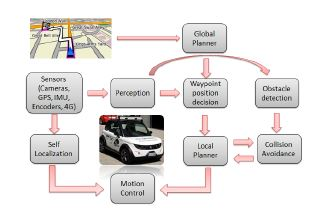
\includegraphics[scale=1.0]{Figure_block_dig}
		\caption{System architecture for autonomous vehicle}
		\label{fig:SysArch}
\end{figure}

\newpage
\section{Modeling for Planning and Control}

\subsection{Kinematic model of a car like robot}


\begin{figure}[!ht]
	\centering
	\includegraphics[scale= 0.5]{vehicle_model.png}
	\caption{Kinematics of a car like mobile robot}
	\label{fig:SysArch}
\end{figure}
 
The differential constraint for rear wheel is given by: 

\begin{eqnarray}
R &= \frac{l}{\tan \delta} \\
\dot{x}_r &= v_r \cos (\theta) \\
\dot{y}_r &= v_r \sin (\theta) \\
\dot{\theta} &= \frac{v_r}{l} \tan \delta \\
\dot{v}_r &= a
\end{eqnarray}

The differential constrain can also be written in terms of motion of forward wheel, 
\begin{eqnarray}
    \dot{x}_f &= v_f \cos (\theta + \delta) \\
    \dot{y}_f &= v_f \sin (\theta \delta) \\
    \dot{\theta} &= \frac{v_f}{l} \tan \delta
\end{eqnarray} 

The front wheel speed $v_f$, is related to rear wheel speed $v_f$ by: 
\begin{equation}
\frac{v_r}{v_f} = \cos (\delta)
\end{equation}

The planning and control problems for this model involve selecting the steering angle $\delta$ within the mechanical limits of the vehicle $\delta \in [\delta_{min}, \delta_{max}]$, and forward speed $v_r$ within an acceptable range, $v_r \in [v_{min}, v_{max}]$ \cite{paden2016survey}.

A simplification that is sometimes utilized is to selected the heading rate $\omega$ instead of the steering angle $\delta$. These quantities are related by 
\begin{equation}
	\delta = \arctan \Big ( \frac{l\omega}{v_r}\Big )
\end{equation}
simplifying the heading dynamics to 

\begin{equation}
	\dot{\theta} = \omega, \quad 
	\omega \in \begin{bmatrix}
 		 \frac{v_r}{l} \tan (\delta_{min}), & \frac{v_r}{l} \tan (\delta_{max})
	\end{bmatrix}
\end{equation}


\section{Vehicle Control}

\section{Trajectory Planning} 

\bibliographystyle{unsrt}
\bibliography{mybib}



\end{document}
